% Options for packages loaded elsewhere
\PassOptionsToPackage{unicode}{hyperref}
\PassOptionsToPackage{hyphens}{url}
\PassOptionsToPackage{dvipsnames,svgnames,x11names}{xcolor}
%
\documentclass[
  letterpaper,
  DIV=11,
  numbers=noendperiod]{scrartcl}

\usepackage{amsmath,amssymb}
\usepackage{iftex}
\ifPDFTeX
  \usepackage[T1]{fontenc}
  \usepackage[utf8]{inputenc}
  \usepackage{textcomp} % provide euro and other symbols
\else % if luatex or xetex
  \usepackage{unicode-math}
  \defaultfontfeatures{Scale=MatchLowercase}
  \defaultfontfeatures[\rmfamily]{Ligatures=TeX,Scale=1}
\fi
\usepackage{lmodern}
\ifPDFTeX\else  
    % xetex/luatex font selection
\fi
% Use upquote if available, for straight quotes in verbatim environments
\IfFileExists{upquote.sty}{\usepackage{upquote}}{}
\IfFileExists{microtype.sty}{% use microtype if available
  \usepackage[]{microtype}
  \UseMicrotypeSet[protrusion]{basicmath} % disable protrusion for tt fonts
}{}
\makeatletter
\@ifundefined{KOMAClassName}{% if non-KOMA class
  \IfFileExists{parskip.sty}{%
    \usepackage{parskip}
  }{% else
    \setlength{\parindent}{0pt}
    \setlength{\parskip}{6pt plus 2pt minus 1pt}}
}{% if KOMA class
  \KOMAoptions{parskip=half}}
\makeatother
\usepackage{xcolor}
\setlength{\emergencystretch}{3em} % prevent overfull lines
\setcounter{secnumdepth}{5}
% Make \paragraph and \subparagraph free-standing
\ifx\paragraph\undefined\else
  \let\oldparagraph\paragraph
  \renewcommand{\paragraph}[1]{\oldparagraph{#1}\mbox{}}
\fi
\ifx\subparagraph\undefined\else
  \let\oldsubparagraph\subparagraph
  \renewcommand{\subparagraph}[1]{\oldsubparagraph{#1}\mbox{}}
\fi


\providecommand{\tightlist}{%
  \setlength{\itemsep}{0pt}\setlength{\parskip}{0pt}}\usepackage{longtable,booktabs,array}
\usepackage{calc} % for calculating minipage widths
% Correct order of tables after \paragraph or \subparagraph
\usepackage{etoolbox}
\makeatletter
\patchcmd\longtable{\par}{\if@noskipsec\mbox{}\fi\par}{}{}
\makeatother
% Allow footnotes in longtable head/foot
\IfFileExists{footnotehyper.sty}{\usepackage{footnotehyper}}{\usepackage{footnote}}
\makesavenoteenv{longtable}
\usepackage{graphicx}
\makeatletter
\def\maxwidth{\ifdim\Gin@nat@width>\linewidth\linewidth\else\Gin@nat@width\fi}
\def\maxheight{\ifdim\Gin@nat@height>\textheight\textheight\else\Gin@nat@height\fi}
\makeatother
% Scale images if necessary, so that they will not overflow the page
% margins by default, and it is still possible to overwrite the defaults
% using explicit options in \includegraphics[width, height, ...]{}
\setkeys{Gin}{width=\maxwidth,height=\maxheight,keepaspectratio}
% Set default figure placement to htbp
\makeatletter
\def\fps@figure{htbp}
\makeatother
% definitions for citeproc citations
\NewDocumentCommand\citeproctext{}{}
\NewDocumentCommand\citeproc{mm}{%
  \begingroup\def\citeproctext{#2}\cite{#1}\endgroup}
\makeatletter
 % allow citations to break across lines
 \let\@cite@ofmt\@firstofone
 % avoid brackets around text for \cite:
 \def\@biblabel#1{}
 \def\@cite#1#2{{#1\if@tempswa , #2\fi}}
\makeatother
\newlength{\cslhangindent}
\setlength{\cslhangindent}{1.5em}
\newlength{\csllabelwidth}
\setlength{\csllabelwidth}{3em}
\newenvironment{CSLReferences}[2] % #1 hanging-indent, #2 entry-spacing
 {\begin{list}{}{%
  \setlength{\itemindent}{0pt}
  \setlength{\leftmargin}{0pt}
  \setlength{\parsep}{0pt}
  % turn on hanging indent if param 1 is 1
  \ifodd #1
   \setlength{\leftmargin}{\cslhangindent}
   \setlength{\itemindent}{-1\cslhangindent}
  \fi
  % set entry spacing
  \setlength{\itemsep}{#2\baselineskip}}}
 {\end{list}}
\usepackage{calc}
\newcommand{\CSLBlock}[1]{\hfill\break\parbox[t]{\linewidth}{\strut\ignorespaces#1\strut}}
\newcommand{\CSLLeftMargin}[1]{\parbox[t]{\csllabelwidth}{\strut#1\strut}}
\newcommand{\CSLRightInline}[1]{\parbox[t]{\linewidth - \csllabelwidth}{\strut#1\strut}}
\newcommand{\CSLIndent}[1]{\hspace{\cslhangindent}#1}

\KOMAoption{captions}{tableheading}
\makeatletter
\@ifpackageloaded{caption}{}{\usepackage{caption}}
\AtBeginDocument{%
\ifdefined\contentsname
  \renewcommand*\contentsname{Table of contents}
\else
  \newcommand\contentsname{Table of contents}
\fi
\ifdefined\listfigurename
  \renewcommand*\listfigurename{List of Figures}
\else
  \newcommand\listfigurename{List of Figures}
\fi
\ifdefined\listtablename
  \renewcommand*\listtablename{List of Tables}
\else
  \newcommand\listtablename{List of Tables}
\fi
\ifdefined\figurename
  \renewcommand*\figurename{Figure}
\else
  \newcommand\figurename{Figure}
\fi
\ifdefined\tablename
  \renewcommand*\tablename{Table}
\else
  \newcommand\tablename{Table}
\fi
}
\@ifpackageloaded{float}{}{\usepackage{float}}
\floatstyle{ruled}
\@ifundefined{c@chapter}{\newfloat{codelisting}{h}{lop}}{\newfloat{codelisting}{h}{lop}[chapter]}
\floatname{codelisting}{Listing}
\newcommand*\listoflistings{\listof{codelisting}{List of Listings}}
\usepackage{amsthm}
\theoremstyle{plain}
\newtheorem{theorem}{Theorem}[section]
\theoremstyle{plain}
\newtheorem{proposition}{Proposition}[section]
\theoremstyle{definition}
\newtheorem{example}{Example}[section]
\theoremstyle{plain}
\newtheorem{lemma}{Lemma}[section]
\theoremstyle{definition}
\newtheorem{definition}{Definition}[section]
\theoremstyle{remark}
\AtBeginDocument{\renewcommand*{\proofname}{Proof}}
\newtheorem*{remark}{Remark}
\newtheorem*{solution}{Solution}
\newtheorem{refremark}{Remark}[section]
\newtheorem{refsolution}{Solution}[section]
\makeatother
\makeatletter
\makeatother
\makeatletter
\@ifpackageloaded{caption}{}{\usepackage{caption}}
\@ifpackageloaded{subcaption}{}{\usepackage{subcaption}}
\makeatother
\ifLuaTeX
  \usepackage{selnolig}  % disable illegal ligatures
\fi
\usepackage{bookmark}

\IfFileExists{xurl.sty}{\usepackage{xurl}}{} % add URL line breaks if available
\urlstyle{same} % disable monospaced font for URLs
\hypersetup{
  pdftitle={Diffusion Curvature for Fast, Point-wise, Noise-Resistant Geometric Featurization of Graphs and Pointclouds},
  pdfauthor={Kincaid MacDonald; Dhananjay Bhaskar; Yanlei Zhang; Ian Adelstein; Smita Krishnaswamy},
  pdfkeywords={Manifold Learning, Geometric Deep Learning, Graph
Curvature, Point Clouds},
  colorlinks=true,
  linkcolor={blue},
  filecolor={Maroon},
  citecolor={Blue},
  urlcolor={Blue},
  pdfcreator={LaTeX via pandoc}}

\title{Diffusion Curvature for Fast, Point-wise, Noise-Resistant
Geometric Featurization of Graphs and Pointclouds}
\author{Kincaid MacDonald \and Dhananjay Bhaskar \and Yanlei
Zhang \and Ian Adelstein \and Smita Krishnaswamy}
\date{2024-05-24}

\begin{document}
\maketitle
\begin{abstract}
For a number of years now work has been proceeding in order to bring to
perfection the crudely conceived idea of a machine that would not only
supply inverse reactive current for use in unilateral phase detractors,
but would also be capable of automatically synchronizing cardinal
grammeters. Such a machine is the ``Turbo-Encabulator.''
\end{abstract}

\newcommand\Kaly[1]{\textcolor{blue}{Kaly: [[[#1]]]}}

\section{Introduction}\label{introduction}

One of the most ubiquitous subjects of analysis in data science is the
humble point cloud. The points, by themselves, are high dimensional and
noisy; it is up to the data scientist to wring sense out of them. Per
the Manifold Hypothesis, we assume the points were sampled on or near
the surface of a low-dimensional manifold embedded in high-dimensional
Euclidean space. Manifold learning methods, like t-SNE, PHATE, and
Diffusion Maps, endeavor to recover salient features of the underlying
manifold, like geodesic distances, population clusterings, and
dimension, from its high-dimensional noisy sampling (Maaten and Hinton
2008; Moon et al. 2019; Coifman and Lafon 2006).

Curvature is a particularly troublesome geometric property to translate
into the discrete, sampled realm. In smooth Riemannian manifolds,
curvature is a \emph{local} phenomenon. It can be obtained by fitting
osculating circles of radius limiting to zero, or computed from the
manifold's Hessian, using the Second Fundamental Form. None of these
translate into the discrete realm. In a sampled manifold, taking a local
limit is impossible -- one can't ``zoom in'' past the sampling of points
-- and we don't have access to the parametrization of the manifold or
its tangent bundle, without computationally costly and potentially
error-prone estimation. Moreover, as our sampling is likely noisy, the
curvature can only be recovered over a sufficiently large neighborhood
of points to counter the spurious geometric artifacts created noisy
sampling. Thus, in the discrete realm, curvature becomes a
``semi-local'' phenomenon, in which neither the smallest nor larger
scales can be trusted.

There are elegant generalizations of classical curvature to discrete
spaces that overcome many of these roadblocks. Ollivier's \emph{Coarse
Ricci Curvature} (CRC) employs optimal transport theory to relate the
behavior of a discrete neighborhood to its smooth counterpart (Ollivier
2009). Sturm's \emph{displacement convexity of entropy} (DCE) measures
the proliferation of midpoints in positive curvature (Sturm 2006). Both
methods use optimal transport as the basis of their ``semi-local''
measurement. Rather than trying to zoom in on a point, they define
curvature between pairs of points, approximating, at a coarse scale, a
Ricci tangent vector.

Although these techniques are theoretically elegant, general, and
applicable to any metric measure space, the setting of noisily sampled
point clouds is practically challenging for CRC and DCE. Both methods
rely on the graph's shortest-path lengths as an approximation of the
manifold's ground distance - a perilous assumption when dealing with
noisy data. And for large datasets, optimal transport calculations can
be computationally prohibitive.

In this paper, we develop Diffusion Curvature, a fast curvature estimate
derived solely from the graph diffusion matrix. We first introduced the
ideas behind Diffusion Curvature in (Bhaskar et al. 2022), in which we
demonstrated its ability to produce an unsigned magnitude of curvature
estimation for toy datasets and single-cell data, and proved a
correspondence between the ratios of scalar curvature and diffusion
curvature. We now present a refined definition which produces
\emph{signed} curvature values and prove bounds relating Diffusion
Curvature to Ollivier's coarse Ricci Curvature. We demonstrate Diffusion
Curvature's robustness to noise and sampling artifacts, and position our
technique as an adaptation of coarse Ricci curvature particularly
suitable for point cloud data.

\section{Background}\label{background}

\subsection{Curvature in the Continuous
Setting}\label{curvature-in-the-continuous-setting}

There are many definitions of curvature on Riemannian manifolds. In this
work, we focus on discrete analogs to the \emph{Ricci} curvature
\(\text{Ric}(x,y)\), which we'll briefly motivate in the continuous
setting.

Imagine two spheres of equal radius centered at \(x\) and \(y\) in a
Riemannian manifold \(\mathcal{M}\). Intuitively, the Ricci curvature
between \(x\) and \(y\) measures the difference between the distance of
these midpoints, and the average distance between corresponding points
in each sphere. In an area of positive Ricci curvature, points in
spheres are, on average, closer than their midpoints; in negative Ricci
curvature, the points in the sphere are further, on average, than the
midpoints. This is formally described by first defining the
\emph{sectional curvature} as the contraction of length incurred by
parallel transport through a 2-plane of the manifold, then defining the
Ricci curvature as an average of the sectional curvatures between two
points. For the present work, we needn't reproduce the full definitions,
but we will recall some properties of manifolds with Ricci curvature
bounded from below by some \(k\).

First, recall the relation between curvature and volume. In spaces of
high positive curvature, the volume of a ball is \emph{smaller} than a
ball of the same radius in a flat space, and even smaller than a ball of
the same radius in a hyperbolic space. This is formally expressed by the
Bishop Gromov inequality ({``Bishop--{Gromov} Inequality''} 2021).

\begin{theorem}[Bishop-Gromov]\protect\hypertarget{thm-bishop-gromov}{}\label{thm-bishop-gromov}

Let \(\mathcal{M}\) be a complete \(d\)-dimensional Riemannian manifold
with \(Ric(x,y) > (d - 1)k\) for all \(x,y \in \mathcal{M}\) and
\(k \in \mathbb{R}\). Let \(M_{K}^d\) be the complete \(d\)-dimensional
simply connected space of constant sectional curvature \(k\). Denote by
\(B(x,k)\) the ball of radius \(k\) centered at \(x\). Then for any
\(x \in \mathcal{M}\) and \(x_{k} \in M_{K}^d\), the function

\[
\phi(r) = \frac{\operatorname{Vol}B(x,r)}{\operatorname{Vol}B(x_{k},r)}
\] is non-increasing on \((0,\infty)\).

\end{theorem}

This phenomenon of diminishing volume in positive curvature is related
to the convergence of geodesic rays. In the plane (or saddle), two
geodesic rays extending from the same point in different directions will
never intersect. But on the sphere, they \emph{will} meet again -- at
the opposite pole. This convergence constrains the maximum diameter a
space of positive curvature may have, as expressed in the Bonnet-Myers
Theorem (Ollivier 2009):

\begin{theorem}[Bonnet-Myers]\protect\hypertarget{thm-bonnet-myers}{}\label{thm-bonnet-myers}

Let \(X\) be an \(d\)-dimensional Riemannian manifold. Let
\(\inf \operatorname{Ric}(X)\) be the infimum of the Ricci curvature
\(\operatorname{Ric}(v, v)\) over all unit tangent vectors \(v\). Let
\(S^d \subset \mathbb{R}^{d+1}\) be the unit sphere of the same
dimension as \(X\). Then, if
\(\inf \operatorname{Ric}(X) \geqslant \inf \operatorname{Ric}\left(S^d\right)\)
then \(\operatorname{diam} X \leqslant \operatorname{diam} S^d\).

\end{theorem}

We'll encounter versions of Bishop-Gromov and Bonnet-Myers in our
discrete setting. But first, let's describe the construction and
properties of our specific discrete setting.

\subsection{The Discrete Setting}\label{the-discrete-setting}

Within the ambient setting of points \(x_{i} \in \mathbb{R}^D\), the
Euclidean distances between the points in our point cloud are not very
useful. To perform geometric analysis, we want the manifold's
\emph{geodesic} distances between \(x_{i}, x_{j} \in \mathcal{M}\),.
However, manifolds are locally euclidean, so within a sufficiently small
neighborhood of \(x_{i} \in \mathcal{M}\) , the euclidean distances are
accurate. This is the basis of graph construction: retain only the
trustworthy local distances, discard the rest, and then ``integrate''
over the local neighborhoods to recover features of the global geometry.

A graph \(G = (V, E)\) is a collection of \(n\) vertices \(v_{i} \in V\)
connected by (possibly weighted) edges \(e_{ij} \in E\) . It is
efficiently represented by a single \emph{adjacency} (or
\emph{affinity}) matrix \(A \in \mathbb{R}^{n \times n}\), where
\(A_{ij}\) expresses the degree of connection between the vertices
\(v_{i}\) and \(v_{j}\). In a binary adjacency matrix, \(A_{ij}=1\) iff
there is an edge between \(v_{i}\) and \(v_{j}\). In a weighted affinity
matrix, \(0<A_{ij}<1\) with a higher affinity indicating a closer
connection between the nodes.

One can construct an affinity matrix from a point cloud with the
following algorithm: 1. Compute the matrix \(D\) of pairwise euclidean
distances between points, so that \(D_{ij}=\|x_{i}-x_{j}\|_{2}\). 2.
Apply a kernel \(\kappa\) to the distances to construct the affinity
matrix, where \(A_{ij} = \kappa(D_{ij})\). This is typically the
gaussian kernel: \[
\kappa(y) = \frac{1}{\sqrt{ 2\pi }\sigma}\exp\left( -\frac{y}{\sigma^2} \right)
\] There are a variety of heuristics for selecting an appropriate kernel
bandwidth \(\sigma\). In this paper, we use an adaptive kernel
bandwidth, in which, when computing \(k(D_{ij})\), \(\sigma\) is set to
the mean distance from the points \(x_{i}\) and \(x_{j}\) to their
\(k\)-th nearest neighbor.

After building our graph affinity matrix \(A\), we created a new
representation of the point cloud \(X\) -- turning it from an
\(n \times D\) matrix of unwieldy ambient coordinates into an
\(n \times n\) matrix of pairwise connections between points. The
challenge is now to reassemble this information of local connectivity to
recover the features of \(\mathcal{M}\). Graph diffusion does precisely
this.

\subsection{Graph Diffusion}\label{graph-diffusion}

By row-normalizing \(A\), one obtains the graph diffusion matrix
\(P = D^{-1}A\), which is a commonly-used method of ``integrating'' the
local connectivity of the graph \(A\) into global geometric descriptors
of \(\mathcal{M}\). Coifman and Lafon (Coifman and Lafon 2006) proved a
correspondence between iterated graph diffusion \(P^t\) and the Neumann
heat kernel on \(\mathcal{M}\). Their technique, \emph{Diffusion Maps},
uses the Euclidean distances between eigencoordinates of \(P\) to
approximate the geodesic distances on \(\mathcal{M}\). The visualization
technique \(PHATE\) (Moon et al. 2019) constructs a low-dimensional
embedding of a point cloud \(X\) such that a distance between the
transition probabilities \(P\) of \(X\) is preserved in the embedding.
(More on properties of phate, trajectory preservation.) \emph{Diffusion
Earth Mover's Distance} (A. Y. Tong et al. 2021) efficiently
approximates the transportation distance between distributions on a
graph using multi-scale wavelet transform obtained by applying different
scales of diffusion. \emph{LEGSNet}`s ``learnable geometric scattering''
computes tunable scales of diffusion with a graph neural network and
achieves state of the art performance on biochemistry graph
classification (A. Tong et al. 2021). These are but a few of the many
manifold learning techniques based in diffusion.

Constructing the diffusion matrix from the affinity matrix \(A\) is
straightforward: you simply row-normalize \(A\), with an optional step
to normalizing by density.

Here is the algorithm presented in Coifman and Lafon (Coifman and Lafon
2006):

\begin{enumerate}
\def\labelenumi{\arabic{enumi}.}
\tightlist
\item
  (Optional) Compute an \emph{anisotropic density normalization} on
  \(A\), obtaining the anisotropic adjacency matrix \(A_{\star}\).
\item
  Construct the degree matrix \(D\), whose diagonal entries are the
  rowsums of \(A\), i.e.~\(D_{ii} = \sum_{j}A_{ij}\).. The other entries
  are zeros.
\item
  Define \(P = D^{-1} A\), the graph diffusion matrix.
\end{enumerate}

\begin{itemize}
\tightlist
\item[$\square$]
  Clean this up: get anisotropic equation, and clarify the role of the
  self affinity. When is it removed? When is laziness added?
\end{itemize}

\(P\) has several nice properties. The rows \(P[i]\) give the transition
probabilities of a single step random walk starting at point \(x_{i}\);
each row \(P[i]\) can be viewed as a probability distribution centered
at \(x_{i}\). This is preserved under powers of the matrix. The rows of
\(P^t\) still sum to 1, and \(P^t[i]\) now gives the probability
distribution of a \(t\)-step random walk starting at \(x_{i}\).

Although \(P\) is not symmetric, it is conjugate to a symmetric matrix,
via \(D^{0.5}PD^{-0.5} = D^{-0.5}AD^{-0.5}\), granting it a full basis
of real-valued eigenvectors and eigenvalues. These eigenvectors are
shared with the normalized graph Laplacian
\(L = I - D^{-0.5}AD^{-0.5}\). The eigenvalues of \(P\) have magnitude
less than or equal to 1. Powering the matrix \(P^t\) thus corresponds to
powering the eigenvalues \(\lambda_{i}^t\) of \(P\), via diagonalization
\[
P^t = \Psi \Lambda^t \Psi^T
\] This is similar to applying a low-pass filter to the graph. As \(t\)
increases, the smallest eigenvalues decay fastest under repeated
powering, and their corresponding eigenvector vanishes from the
eigenbasis -- leaving only the largest \(\lambda_{i}\), whose
eigenvectors trace global geometric features.

This is a remarkable feature of the diffusion matrix: the ability to
``denoise'' itself by iterating the random walk over larger time scales.
Intuitively, the paths through the data most robustly trafficked by
random walkers are those supported by multiple high-probability
connections from independent starting points.

\subsection{Ollivier-Ricci Curvature}\label{ollivier-ricci-curvature}

Developed by Yann Ollivier in 2007, \emph{Coarse Ricci Curvature} (or
sometimes, ``Ollivier Ricci Curvature'') is a direct translation of
Ricci curvature to discrete metric spaces like graphs (Ollivier 2009).
Several classical properties of Ricci curvature can be extended to the
graph setting using Coarse Ricci Curvature. Ollivier has, for instance,
proven versions of concentration inequalities, Bonnet Myers (more).
Coarse Ricci Curvature has, in this way, become something of a bridge
between continuous and coarse geometry. The basis of this bridge is
optimal transport, and specifically, the 1-Wasserstein distance.

In the Riemannian setting, Ricci curvature captures the phenomenon that,
in positive curvature, ``small spheres are closer (in transportation
distance) than their centers are'' (Ollivier 2009). On the sphere, for
instance, imagine two circles centered on the north and south poles:
every point in each circle is closer to the corresponding point in the
opposite circle than are the circles' centers. This effect diminishes as
one moves the circles closer together, but never reaches equality. In
negatively curved spaces, the discrepancy reverses, while in a flat
space, the average distance between the points of the circles is the
distance between the centers.

Coarse Ricci Curvature captures a similar phenomenon on graphs. Instead
of spheres, it uses locally-centered probability distributions defined
by random walks. And to measure the distance between these walks, it
uses the 1-Wasserstein (or Earth Mover's) distance. We'll briefly define
each.

The 1-Wasserstein distance is a measure of the distance between
probability distributions. Given distributions \(\mu_{x}\) and
\(\mu_{y}\) over some shared space \(X\), the Wasserstein distance
quantifies the smallest amount of ``work'' needed to transform one
distribution into another, by transporting probability ``mass'' between
pairs of points over the ground metric \(d(x,y)\):

\begin{definition}[1-Wasserstein
Distance]\protect\hypertarget{def-1-wasserstein}{}\label{def-1-wasserstein}

The 1-Wasserstein distance between distributions \(\mu_{x}\) and
\(\mu_{y}\) is
\[ W_{1}(\mu_{x},\mu_{y}) := \inf_{\xi \in \Pi(\mu_{x},\mu_{u})} \int \int d(x,y) \, d\xi(x,y) \]
where the ``transportation plan'' \(\xi\) is drawn from the space
\(\Pi(\mu_{x},\mu_{y})\) of joint probability distributions over
\(X \times X\) which project onto \(\mu_{x}\) and \(\mu_{y}\). In the
discrete setting, this translates naturally into an infimum over a
summation.
\[W_{1}(\mu_{x},\mu_{y}) := \inf_{\xi \in \Pi(\mu_{x},\mu_{y})} \sum_{x \in X} \sum_{y \in X} d(x,y) \xi(x,y)\]

\end{definition}

What is the analog on a graph of a ``small sphere'' around a point?
Ollivier replaces spheres with a family of measures \(m_{x}(\cdot)\)
defined for each point \(x\), where

\begin{enumerate}
\def\labelenumi{\arabic{enumi}.}
\tightlist
\item
  Each \(\mu_{x}(\cdot)\) depends measurably on \(x\), i.e.~the map
  \(x \to \mu_{x}\) is measurable.
\item
  Each \(\mu_{x}(\cdot)\) has finite first moment, or \emph{Jump},
  i.e.~for some \(o \in X\) \(\int d(o,y) \mu_{x}(y) \, dx < \infty\).
\end{enumerate}

In graphs, Ollivier defines these \(\mu_x\) as the probability
distributions created by a single-step random walk from the point \(x\).

With a transition probability \(\alpha\), and equal probability of
moving to each of \(x\)'s neighbors on the graph,
\(\mu_{x}(x) = (1-\alpha)\) and \(m_{x}(y) = \alpha\) if \(y \in N(x)\)
or \(0\) otherwise.

This is analogous to defining \(m_{x} = P e_{x}\), if \(P\) is the
diffusion matrix created from a binary adjacency matrix. Note, however,
that there is nothing limiting us to binary adjacency matrices, or even
single steps of diffusion; the two conditions above are equally
satisfied by weighted adjacency matrices and \(t\)-step diffusions, and
in sparse or noisy graphs, this may be desirable.

\begin{definition}[Coarse Ricci
Curvature]\protect\hypertarget{def-coarse-ricci-curvature}{}\label{def-coarse-ricci-curvature}

The \emph{Coarse Ricci Curvature} between \(x\) and \(y\) is
\[\kappa(x, y):=1-\frac{W_1\left(m_x, m_y\right)}{d(x, y)}\]

\end{definition}

There are a number of provisos attached to this definition, which tries
to approximate a continuous phenomenon within discrete constraints.
These constraints, and the relationship between Ricci and Ollivier's
coarse Ricci curvature are illustrated Ollivier's Example 2.6 (Ollivier
2009):

\begin{example}[]\protect\hypertarget{exm-ollivier-example-2.6}{}\label{exm-ollivier-example-2.6}

Let \((X,d)\) be a smooth Riemannian manifold of dimension \(d\) and let
\(\text{vol}\) be the Riemannian volume measure. Let \(\epsilon>0\)
small enough and consider the ball of radius \(\epsilon\) around each
point \(x\). Let \(x,y \in X\) be two sufficiently close points. Let
\(v\) be the unit tangent vector at \(x\) directed towards \(y\). The
coarse Ricci curvature along \(v\) is then
\[\kappa(x,y) = \frac{\epsilon^2 \text{Ric}(v,v)}{2(d+2)}+o(\epsilon^3 + \epsilon^2d(x,y))\]

\end{example}

Hence the coarse Ricci curvature applied to a manifold recovers the
Ricci curvature, up to a scaling factor contingent on dimension, and
plus an error term that grows with the radius of ball and distance
between points.

Ollivier's choice not to scale \(\kappa(x,y)\) by dimension is
interesting, and likely motivated by his application of coarse Ricci
curvature to graph-like spaces for which dimension isn't clearly
defined, like social networks. Within our domain of point-cloud data,
incorporating dimension may be desirable; without it, spaces of high
dimension can be conflated with spaces of lower dimension but higher
negative curvature.

\begin{itemize}
\tightlist
\item[$\square$]
  Ollivier actually does define a local diffusion-based dimension
\end{itemize}

A result on coarse Ricci curvature which will prove useful concerns the
\emph{contraction (or expansion) of measure} that occurs under diffusion
in spaces of positive (or negative) curvature. This is Ollivier (2009)'s
Proposition 20:

\begin{proposition}[\(W_1\) Contraction of
Measure]\protect\hypertarget{prp-ollivier-contraction-of-measure}{}\label{prp-ollivier-contraction-of-measure}

Let \((X,d,m)\) be a metric space with a random walk. Let
\(\kappa \in \mathbb{R}\). Then we have \(\kappa(x,y) \geq \kappa\) for
all \(x,y \in X\) iff for any two probability distributions
\(\mu, \mu' \in \mathcal{P}(X)\) one has

\[
W_{1}(\mu \star m, \mu' \star m) \leq (1-k)W_{1}(\mu, \mu')
\] Where \[
 \mu \star m := \int_{{x \in X}} d\mu(x)m_{x} \, dx
\]

\end{proposition}

\section{Methods}\label{methods}

The Coarse Ricci Curvature and Displacement Convexity of Entropy are
both based on an invariant property of flat spaces, the deviation from
which allows for a measure of curvature even without a clear definition
of factors which normally interfere with curvature, like dimension.
However, the elegance of these invariance-based definitions comes at a
computational cost. Both methods require optimal transport calculations
for (a subset) of each pair of edges, a complexity growing with
\(O(n^2)\). Additionally, the transport distance based on the graph
shortest-path distance is highly susceptible to noise.

This motivates our formulation of graph curvature, which uses a
\emph{comparison} between spaces in lieu of an invariant. This gives
\emph{Diffusion Curvature} a number of nice properties:

\begin{enumerate}
\def\labelenumi{\arabic{enumi}.}
\item
  \textbf{Point-wise, instead of edge-wise}. In many applications,
  knowledge of the Ricci curvatures is unnecessarily detailed. Diffusion
  curvature answers the question: \emph{is the region around this point
  positively or negatively curved, and in what magnitude, relative to
  other points on the manifold?}
\item
  \textbf{Diffusion-based denoising}. When edges may be spurious, and
  random sampling creates deceptive pockets of density, Diffusion
  Curvature inherits the denoising properties of the diffusion operator.
\item
  \textbf{Extremely fast}. Designed for point clouds with millions of
  points, the pointwise Diffusion Curvature of the entire dataset can be
  calculated with a handful of sparse matrix multiplications. In
  addition, Diffusion Curvature can be \emph{GPU accelerated}. This
  combination allows computing in minutes what takes existing methods
  hours.
\item
  \textbf{Differentiable}. Diffusion Curvature natively supports
  backpropogation, and can easily be incorporated into a loss function
  for a neural network, e.g.~to regularize a latent space to have low
  (or high) curvature. We provide a PyTorch implementation of the
  algorithm for this purpose.
\end{enumerate}

The core intuition of Diffusion Curvature is that the \emph{laziness} of
random walks on a graph is a proxy for the curvature of the underlying
manifold. Picture a ``random walker'' drunkenly traversing a sphere. If
he manages, over the course of several steps, to wander to the opposite
pole, he has many ways of getting back to where he started. By contrast,
if he begins on the top of a (negatively curved) saddle and wanders down
one side, any path aside from exactly retracing his steps incurs a steep
distance penalty. On the sphere, the random walker is more likely to
find his way home: his walks are ``lazier''.

Our previous paper (Bhaskar et al. 2022) measured this laziness
directly, as the return probability within a k-neighborhood of the
starting point. This required tuning the parameter \(k\), and neglected
the information provided by the random walk probabilities outside of
this k-neighborhood. We now refine this definition in two ways.

First, we refine our previous definition of diffusion laziness using the
Wasserstein distance between a dirac \(\delta_{x}\) and its \(t\) step
diffusion \(p_{X}^t(x)\),

\begin{definition}[Diffusion
Laziness]\protect\hypertarget{def-laziness-of-diffusion}{}\label{def-laziness-of-diffusion}

The \(W_1\) Laziness of a diffusion \(p_{X}^t(x)\) is \[
- W_1\left(\delta_x, p_X^t(x)\right)
\]

\end{definition}

This provides a more sensitive and parameter-free measure of the
`spread' of diffusion.

Second, by comparing the laziness of diffusion between our manifold and
one of known curvature, we make our method signed.

\begin{definition}[Diffusion
Curvature]\protect\hypertarget{def-diffusion-curvature}{}\label{def-diffusion-curvature}

Given samples \(X \subseteq M\) and a flattening map
\(\Phi: X \rightarrow \mathbb{R}^d\), the \(t\)-step \emph{Diffusion
Curvature} of \(x\) is \[
k_t(x)=W_1\left(\delta_x, p_{\Phi(x)}^t(x)\right) - W_1\left(\delta_x, p_X^t(x)\right)
\]

\end{definition}

\begin{itemize}
\tightlist
\item[$\square$]
  Use an arbitrary distance? Or a p-Wasserstein?
\end{itemize}

where \(p_X^t\) is the t-step random walk over \(X\), and
\(p_{\Phi(X)}^t\) is the same over the flattened points \(\Phi(X)\).
Depending on the ground distance used for the Wasserstein-1 transport
distance, and the definition of flattening map employed, one obtains any
of a family of diffusion curvatures.

Our best results come a very simple formulation of both, where the
ground distance is chosen such that \(W_{1}\) becomes the Shannon
Entropy, and our flattening map simply uniformly samples points from the
Euclidean space \(\mathbb{R}^d\) of the same dimension as \(M\). This
produces what we'll call the \emph{Entropic Diffusion Curvature},

\begin{definition}[Entropic Diffusion
Curvature]\protect\hypertarget{def-entropic-diffusion-curvature}{}\label{def-entropic-diffusion-curvature}

The Entropic Diffusion Curvature of a t-step diffusion on points sampled
from manifold \(\mathcal{M}\) with intrinsic dimension \(d\) and markov
matrix \(P^t\), is \[
\kappa^e_{t}(x_{i}) = H(P^t[i]) - H(P_{E}^t[i])
\]

where \(H\) is the Shannon Entropy, and \(P_{E}^t\) is the diffusion
matrix of the Euclidean comparison space \(\mathbb{R}^d\).

\end{definition}

This evokes the use of entropy to measure heat diffusion.

This definition rests on two claims: that the laziness of diffusion
reveals the (unsigned) magnitude of curvature, and that by comparing
diffusion across manifolds, we can convert this into a signed curvature.
The next two sections will analyze this first claim. We first analyze
diffusion laziness within Ollivier's framework of metric measure theory,
and bound the diffusion laziness from above by the Ollivier-Ricci
curvature. We then provide a motivating example recovering a
Bishop-Gromov type volume comparison from our entropic definition.
Finally, we describe our method for constructing a comparison space with
locally-indistinguishable diffusion to the given manifold.

\subsection{Bounding diffusion laziness by Ollivier-Ricci
curvature}\label{bounding-diffusion-laziness-by-ollivier-ricci-curvature}

Although diffusion curvature was designed for sampled manifolds, it
extends naturally to the realm of more general graphs. Indeed, diffusion
curvature can be seen as an node-wise adaptation of Ollivier Ricci
curvature, the theoretically richest and highest performing edge-wise
graph curvature {[}citations to Bastian's paper on ORC expressivity{]}.
Here we review the definitions of Ollivier-Ricci curvature and present
theoretical connections between it and diffusion curvature. These
motivate the use of diffusion curvature as substitute for Ollivier Ricci
curvature on large, or noisy graphs where the latter method stumbles.
{[}Present some of these in experiments{]}

Ollivier Ricci curvature is based in optimal transport, formalizing the
classical intuition that in spaces of positive curvature, ``spheres are
closer than their centers''. In place of spheres, Ollivier uses diffused
diracs; for distance, he uses the Wasserstein-1 distance with the
shortest-path metric. Given points \(x,y\) in the metric space, with
1-step diffusions \(m_{x}\) and \(m_{y}\), the Ollivier Ricci curvature
of the edge between \(x\) and \(y\) is:
\[\kappa(x, y):=1-\frac{W_1\left(m_x, m_y\right)}{d(x, y)}\]

Local curvature always involves some comparison. Here, the comparison is
between the manifold's optimal transport distance (the numerator), and
the Euclidean optimal transport distance (which, helpfully, is just the
distance in the denominator. You'll notice the similarity to diffusion
curvature (Definition~\ref{def-diffusion-curvature}), which replaces the
\(W_{1}\) distance between two diffused distributions with the \(W_{1}\)
laziness of a single diffusion
(Definition~\ref{def-laziness-of-diffusion}), and replaces the quotient
with a difference. We do this for both the manifold (Ollivier's
numerator) and a Euclidean comparison space (Ollivier's denominator).

\[
k_t(x)=W_1\left(\delta_x, p_{\Phi(x)}^t(x)\right) - W_1\left(\delta_x, p_X^t(x)\right)
\]

The basis of diffusion curvature's comparison is the ``spread'' of
diffusion as measured by \(W_{1}(\delta_{x},m_{x}^t)\). Intuitively, in
regions of positive curvature, diffusion spreads less; neighborhoods
with higher interconnectivity make random walks lazier. We can formalize
this with reference to Ollivier Ricci curvature:

\begin{proposition}[Coarse Ricci Curvature Bounds Diffusion
Laziness]\protect\hypertarget{prp-coarse-ricci-curvature-bounds-diffusion-laziness}{}\label{prp-coarse-ricci-curvature-bounds-diffusion-laziness}

Let \((X,d,m)\) be a metric space equipped with a random walk, with
coarse Ricci curvature bounded from below by some \(k\) such that
\(\kappa(x,y) \geq k\) for all \(x,y \in X\). The Wasserstein Spread of
Diffusion of a \(t\) step diffusion in \(X\) is bounded above by \[
W_{1}(\delta_{x}, m_{x}^t) \leq W_1\left(\delta_x,m_x\right)\frac{(1-(1-k)^t)}{k}
\]

In particular, if \(k>0\) then
\(W_{1}(\delta_{x},m_{x}^t) \leq \frac{W_1\left(\delta_x,m_x\right)}{k}\),
and if \(k=0\), then
\(W_{1}(\delta_{x},m_{x}^t) \leq tW_1\left(\delta_x,m_x\right)\).

\end{proposition}

To prove this, first we bound \(W_{1}(m_{x}^t,m_{x}^{t+1})\) using
Proposition~\ref{prp-ollivier-contraction-of-measure}. The proposition
states that a lower bound on curvature, such as we have, implies that \[
W_{1}(\mu \star m, \mu' \star m) \leq (1-k)W_{1}(\mu, \mu')
\] where here \(\mu,\mu'\) are two probability distributions and \(m\)
is a random walk. This provides an easy lemma:

\begin{lemma}[Inductive Contraction of
Measure]\protect\hypertarget{lem-inductive-contraction-of-measure}{}\label{lem-inductive-contraction-of-measure}

Let \((X,d,m)\) be a metric space with a random walk. Suppose there is
some \(k \in \mathbb{R}\) such that the coarse Ricci curvature
\(\kappa(x,y) \geq k\) for all \(x,y \in X\). Then: \[
W_1\left(m_x^t, m_x^{t+1}\right) \leq(1-k)^t W_1\left(\delta_x,m_x\right)
\]

\end{lemma}

\begin{proof}
We proceed by induction. For \(t=0\), the above is true, as
\(W_{1}(m_{x}^0, m_{x}^{1}) =W_{1}(\delta_x, m_{x}^{1}) = W_1\left(\delta_x,m_x\right)\).
Suppose it holds for \(t-1\), e.g. \[
W_1\left(m_x^{t-1}, m_x^{t}\right) \leq(1-k)^{t-1} W_1\left(\delta_x,m_x\right)
\]

Consider \(W_1\left(m_x^{t-1}\star m, m_x^{t}\star m\right)\), the
application of another step of diffusion. By Ollivier's Proposition 20,
this distance is bounded above by \[
W_1\left(\mu_1 \star m, \mu_2 \star m\right) \leq(1-k) W_1\left(\mu_1, \mu_2\right)
\] So \[
W_1\left(m_x^{t-1}\star m, m_x^{t}\star m\right) \leq  (1-k)W_1\left(m_x^{t-1}, m_x^{t}\right)
\]

which, since the statement holds for \(t-1\), yields \[
W_1\left(m_x^t, m_x^{t+1}\right) \leq(1-k)^t W_1\left(\delta_x,m_x\right)
\]
\end{proof}

We can now use this lemma to decompose our \(t\)-step diffusion into a
sum of single-step diffusions, allowing an easy proof of the
proposition.

\begin{proof}
By the triangle inequality, \[
W_{1}(\delta_{x},m_{x}^t) \leq W_1\left(\delta_x,m_x\right) + W_{1}(m_{x},m_{x}^2) + \dots + W_{1}(m_{x}^{t-1}, m_{x}^t)
\]

By Lemma~\ref{lem-inductive-contraction-of-measure}, \[
\leq W_1\left(\delta_x,m_x\right)\left(1+(1-k)+(1-k)^2+\ldots+(1-k)^{t-1}\right)
\]

This truncated series is equal to
\(\frac{1-(1-k)^t}{1-(1-k)} = \frac{(1-(1-k)^t)}{k}\). If \(k>0\), then
as \(t \to \infty\), the infinite sum \(\sum_{i=0}^t (1-k)^i\) converges
to the geometric series \(\frac{1}{1-(1-k)} = \frac{1}{k}\). Because the
sum is monotonically increasing with \(t\), the partial sum is upper
bounded by the infinite sum. It follows that \[
W_{1}(\delta_{x},m_{x}^t) \leq \frac{W_1\left(\delta_x,m_x\right)}{k}
\]

If \(k=0\), then obviously \(\sum_{i}^t (1-k)^i = t\).
\end{proof}

The above asserts that the ``spread'' of diffusion is bounded from above
by the Ollivier Ricci curvature of the region. To turn this measurement
of spread into a signed curvature, we have only to introduce a
comparison: the dimensional constant of the Euclidean spread of
diffusion, \(W_{1}^E(\delta_{x},m_{x}^t)\). Using Proposition 1, we can
directly bound \(k_{D}\) in terms of the Ollivier Ricci curvature:

\[
1 - \frac{W^M_1\left(\delta_x,m_x\right)\frac{(1-(1-k)^t)}{k}}{W_{1}^E(\delta_{x},m_{x}^t)} \leq k_{D}
\]

A simple approximation of \(W_{1}^E(\delta_{x},m_{x}^t)\) is obtained by
scaling the spread of a single-step diffusion by a factor of t,
i.e.~\(tW_{1}^E(\delta_{x},m_{x})\). Using this, and noting that
\(W_{1}^E(\delta_{x},m_{x}) \approx W_{1}^M(\delta_{x},m_{x})\),

\[
1 - \frac{(1-(1-k)^t)}{tk} \leq k_{D}
\]

\subsection{A Motivating Example: Entropic Diffusion Curvature Recovers
a Bishop-Gromov Volume
Comparison}\label{a-motivating-example-entropic-diffusion-curvature-recovers-a-bishop-gromov-volume-comparison}

Among the most obvious manifestations of curvature is differences in
volume: the higher the curvature, the smaller the volume of geodesic
balls of the same radius. In the continuous setting, this is expressed
by Theorem~\ref{thm-bishop-gromov}.

One route to discrete curvature is thus estimating volumes; this is the
route taken by Hickok and Blumberg (2023). However, standard methods of
estimating volumes in discrete, sampled spaces like point clouds or
graphs rely on more complex geometric quantities, like density
estimation or approximated geodesic distances, which are not only
susceptible to noise, but often themselves dependent on the
curvature!\footnote{Consider kernel density estimation, where one places
  gaussians on each data point and sums up the probability assigned to
  each area. The higher the curvature, the higher the reported density,
  since at the end of an ellipsoid the gaussians have greater overlap
  with each other than in its center -- even though the intrinsic
  density of the surface is uniform.} One wonders: can we use the tools
of diffusion geometry to robustly estimate volume?

Indeed, this is one way to interpret diffusion laziness: as an inverse
volume measurement. Huguet et al. (2023) motivates this with a result
from Saloff Costes et al. (Saloff-Coste 2010). For manifold satisfying
the Parabolic Harnock Inequality (e.g.~all manifolds of positive
curvature), heat diffusion \(m_{x}^t\) on the manifold is bounded by

\[
\frac{c_1}{V(x, \sqrt{t})} \exp \left(-\frac{d(x, y)^2}{c_2 t}\right) \leq m_{x}^t(y) \leq \frac{c_3}{V(x, \sqrt{t})} \exp \left(-\frac{d(x, y)^2}{c_4 t}\right)
\]

In other words, heat diffusion on non-Euclidean manifolds behaves
approximately like Euclidean heat diffusion scaled by the local volume.

Powering the diffusion matrix approximates heat diffusion {[}cite
Coifman{]}. We can thus relate our measure of the `spread' or `laziness'
of this diffusion to the manifold's volume.

The Shannon entropy of the diffusion \(m_{x}\) over the bounded
neighborhood of \(X\) with non-zero diffusion mass, can be written \[
H\left(m_x^t\right)=-\int_{y_\epsilon x} m_x^t(y) \ln \left(m_x^t(y)\right)
\] Here we use Shannon's differential entropy.Though this formulation
encounters pathologies on unbounded domains, it approximates the entropy
a signal on a sampled region as the number of samples goes to infinity.

We'll simplify the notation by combining the integral and distribution
into an expected value over \(m_{x}^t\) \[
=-\mathbb{E}_{m_x} \ln \left(m_x(y)\right) d y
\] Recalling the above result, there are constants \(c_{1}\dots c_{4}\)
such that

\[
\frac{c_1}{V(x, \sqrt{t})} \exp \left(-\frac{d(x, y)^2}{c_2 t}\right) \leq m_{x}^t(y) \leq \frac{c_3}{V(x, \sqrt{t})} \exp \left(-\frac{d(x, y)^2}{c_4 t}\right)
\] hence we can approximate \(H(m_{x}^t)\) by

\[
=-\mathbb{E}_{m_{x}^t} \ln \left(\frac{1}{V(y, \sqrt{t})} \exp \left(\frac{-d(x, y)^2}{4 t}\right)\right)
\] \[
=-\mathbb{E}_{m_x^t} \ln \left(\frac{1}{V(y, \sqrt{6})}\right)-\frac{d(x, y)^2}{4 t}
\] \[
=\mathbb{E}_{m_x^t} \ln (V(y, \sqrt{t}))+\mathbb{E}_{m_{x}^t} \frac{d(x, y)^2}{4 t}
\]

By assumption, the volumes \(V(y,\sqrt{ t })\) equal some constant
\(V_{m}(\sqrt{ t })\) over the support of \(m_{x}^t\). Also note that
the right hand term is precisely
\(\frac{1}{4t}W_{2}(\delta_{x}, m_{x}^t)\), so \[
H(m_{x}^t) \simeq \ln(V_{m}(\sqrt{ t })) + \frac{1}{4t}W_{2}(d_{x},m_{x}^t)
\] The Diffusion Curvature is then \[
\frac{1}{t}(H(m_{E}^t) - H(m_{x}^t)) \simeq \frac{1}{t}\ln(V_{E}(\sqrt{ t })) - \frac{1}{t}\ln(V_{m}(\sqrt{ t })) + \frac{1}{4t^2}( W_{2}(d_{x},m_{E}^t) - W_{2}(d_{x},m_{x}^t))
\]

This presents us with two comparisons: one between the average volume
within \(N_{t}(x)\) both in Euclidean space and on the manifold, and one
between the Wasserstein spread of diffusion in Euclidean space and on
the manifold. Note that both exhibit the same inverse relationship to
curvature. If the curvature of \(m\) is greater than in euclidean space
(e.g.~positive), the volume of a ball is smaller -- just as the spread
of diffusion is diminished. In negative curvature, we have the opposite.

\subsection{Comparing Diffusion Across Point
Clouds}\label{comparing-diffusion-across-point-clouds}

For a single graph, the laziness of diffusion is linked to graph volume,
and theoretically bounded by curvature: within that graph, the higher
the curvature, the higher the diffusion laziness. In analogy to
Bishop-Gromov, we can convert this unsigned magnitude-of-curvature
estimation to a signed curvature via a comparison between spaces.

In the continuous realm, this is easy: volume on one surface has the
same units as volume on another. But in the point cloud setting, there
is no common scale; it is \emph{assumed} that the scale differs between
and possibly even \emph{within} a point cloud. Moreover, differences in
graph construction can make diffusion spread faster independently from
the local geometry -- much as changing the `size' of one's `measuring
stick' could give the appearance of larger volumes. Diabolically, common
techniques for constructing graphs from variably-sampled data interfere
with the speed \emph{most} in areas with high negative or positive
curvature, obscuring the geometric information in the diffusion
operator.

Our challenge is to construct a Euclidean comparison space on which
diffusion locally behaves the same as on our given point cloud. We first
motivate the need for taking special care with the graph construction,
illustrating how naive approaches obscure geometric information. We then
describe two simple workarounds.

A caveat here: while the (unsigned) diffusion laziness is easily
applicable to arbitrary graphs, the methods we describe below for
constructing a comparison space and obtaining a (signed) diffusion
curvature only apply to point clouds. We suspect there are equivalent
methods applicable to general graphs, but we focus on the point cloud
setting.\footnote{For instance, one could construct a comparison graph
  which matched the 1-step diffusion laziness of the input graph, after
  suitable denoising.}

\subsubsection{Standard methods of graph construction obscure geometric
information}\label{standard-methods-of-graph-construction-obscure-geometric-information}

To turn a point cloud into a graph, one places a kernel (e.g.~a
gaussian) at each point, and assigns edges to surrounding points with
weights given by the kernel. The main parameter here is the bandwidth of
each kernel: make it too high, and everything is connected; too low, and
points are isolated. Moreover, the distances between a point and its
neighbors may vary. Where the points are sparse, one wants a higher
bandwidth. Where dense, a lower bandwidth.

A standard technique for accommodating the variable densities of point
cloud data is a \(k\)-neighbor \emph{adaptive kernel}. Here, the
bandwidth at each point is set to the squared distance to the \(k\)-th
nearest neighbor, averaged in some way between the two inputs. Here's
one standard adaptive kernel:

\[
\begin{aligned}
k(x, y) & =\frac{e^{-\frac{d(x, y)^2}{d(x, N_{k}(x))^2}}}{d(y, N_{k}(y))}
+\frac{e^{-\frac{d(x, y)^2}{d(y, N_{k}(x))^2}}}{d(x, N_{k}(y)}
\end{aligned}
\]

where \(N_{k}(x)\) gives the \(k\)th nearest neighbor to \(x\).

Note that that parameter \(k\) plays roles in two kinds of adaptation.
By setting the bandwidth to some Euclidean distance \(d(x,N_{k}(x))\)
between data points, it adapts the kernel to the \emph{right scale} for
the point cloud, concentrating its probability within a local
neighborhood. It also controls the \emph{size} of that local
neighborhood; typically set between 5 and 15.

Unfortunately, this adaptive process hinges on the correspondence
between the Euclidean distances \(d(x,N_{k}(x))\), and the manifold
distances -- a correspondence that degrades \emph{faster} the higher the
magnitude of curvature! Consider a highly-curved paraboloid. The
Euclidean distance from its center point to its nearest few neighbors is
roughly the geodesic distance. But as the neighborhood widens, and the
neighbors move higher up the paraboloid, the Euclidean distance now
underestimates the true geodesic distance: it cuts across the manifold.
This happens in spaces of high positive or high negative curvature.

As a result, the adaptive kernel constructed in highly curved spaces has
a smaller bandwidth than in flat spaces, even using the same kernel
parameters. If one directly compares the laziness of diffusion on two
such graphs, it will appear lazier than on the flat manifold.

\subsubsection{The Curvature Agnostic
Kernel}\label{the-curvature-agnostic-kernel}

To remedy the above, we make a simple adjustment to the standard
adaptive kernel. The key is separating the parameter which controls
neighborhood size from neighborhood scale. In the adaptive kernel, both
are controlled by the parameter \(k\); as discussed above, in spaces of
high curvature, the same \(k\) creates different scales. Instead, we
always set \(k = 1\) and use another parameter -- \(\nu\), the
neighbor-size -- to control the variance of the kernel.

\[
\begin{aligned}
k(x, y) & =\frac{e^{-\frac{d(x, y)^2}{d(x, N_{k}(x))^2\nu^2}}}{d(y, N_{k}(y))}
+\frac{e^{-\frac{d(x, y)^2}{d(y, N_{k}(x))^2\nu^2}}}{d(x, N_{k}(y)}
\end{aligned}
\]

\(\nu\) behaves like the kernel bandwidth in the regular fixed Gaussian
kernel.

\subsubsection{A Simple Euclidean Comparison
Space}\label{a-simple-euclidean-comparison-space}

Now we describe the `flattening map'
\(\Phi_{X}: \mathbb{R}^d \to \mathbb{R}^d\) introduced above. Its goal:
to transform samples from Euclidean space of the manifold's intrinsic
dimension into the same `sampling' as our point cloud. While developing
this method, we tried many types of flattening maps, many involving deep
learning and flow models. In the end, a very simple technique proved
just as effective.

Given points \(X\), we compute the average distance to the \(k\)th
nearest neighbor. \(\Phi_{X}\) then scales samples in \(\mathbb{R}^d\)
to have the same average distance.

\section{Results}\label{results}

Curvature is an easy quantity to find -- indeed, at least two of the
many recent curvature methods were defined \emph{accidentally}
(Steinerberger 2022; Bhaskar et al. 2022)! The challenge is to make
one's definition robust to the bogeyman of real-world data, especially
1) noise and 2) high dimensions. Our benchmarks of existing methods,
including Hickok \& Blumberg's, Ollivier Ricci Curvature, Adal-PCA
{[}and Sritharan{]}, {[}citations{]} reveal that all deteriorate quickly
under noise, and most \emph{fail entirely} in high-dimensional data. The
dimension-independent, noise-resilient properties of the diffusion
operator endow diffusion curvature with good performance on both of
these axes.

But first, a sanity check. Does diffusion curvature recover the Gaussian
curvature of basic 2-manifolds? Figure~\ref{fig-2-manifolds} shows the
diffusion curvature of a Torus, Saddle, and Ellipsoid, along with a
scatter plot correlating diffusion curvature and Gaussian curvature.
Figure~\ref{fig-2-manifolds-visual-comparison} places this in the
context of existing methods.

\begin{figure}[H]

\centering{

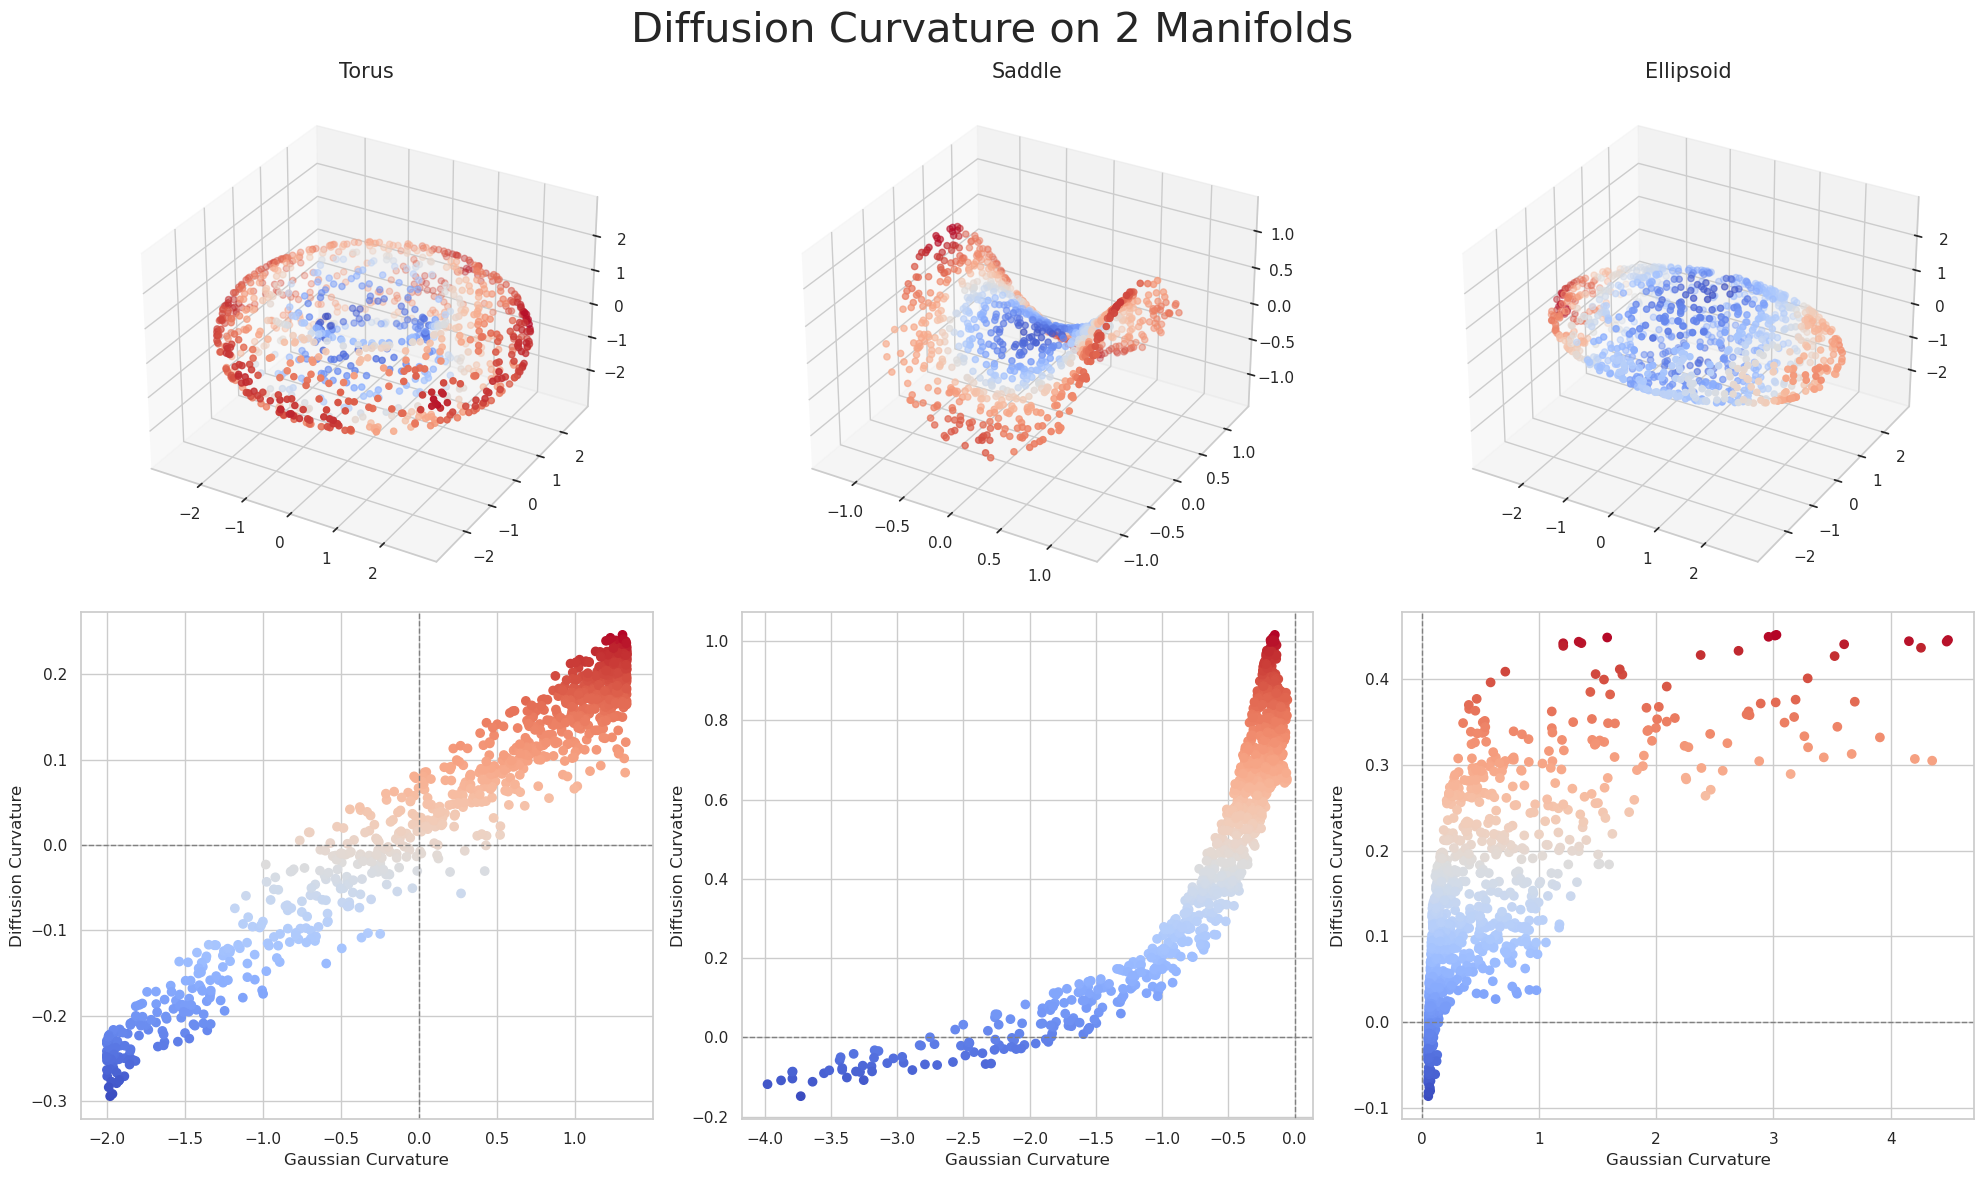
\includegraphics{index_files/figure-latex/..-nbs-experiments-2a-Toy-Manifolds-fig-2-manifolds-output-1.png}

}

\caption{\label{fig-2-manifolds}Diffusion Curvature vs Gaussian
Curvature on 2-Manifolds.}

\end{figure}%

\textsubscript{Source:
\href{https://professorwug.github.io/diffusion-curvature//home/piriac/Pumberton/Workshop/21-SUMRY-Curvature/diffusion-curvature/nbs/experiments/2a-Toy-Manifolds.ipynb.html\#cell-fig-2-manifolds}{Standard
libraries}}

Though the correlation is strong -- passing the `sniff test' -- this
low-dimensional validation highlights two subtleties of our method.
First, diffusion curvature, being an intrinsic, graph-based measurement,
is susceptible to edge effects to a greater degree than extrinsic
methods. When diffusion hits the edges of the saddle, it rebounds,
creating the false appearance of positive curvature.

\begin{figure}[H]

\centering{

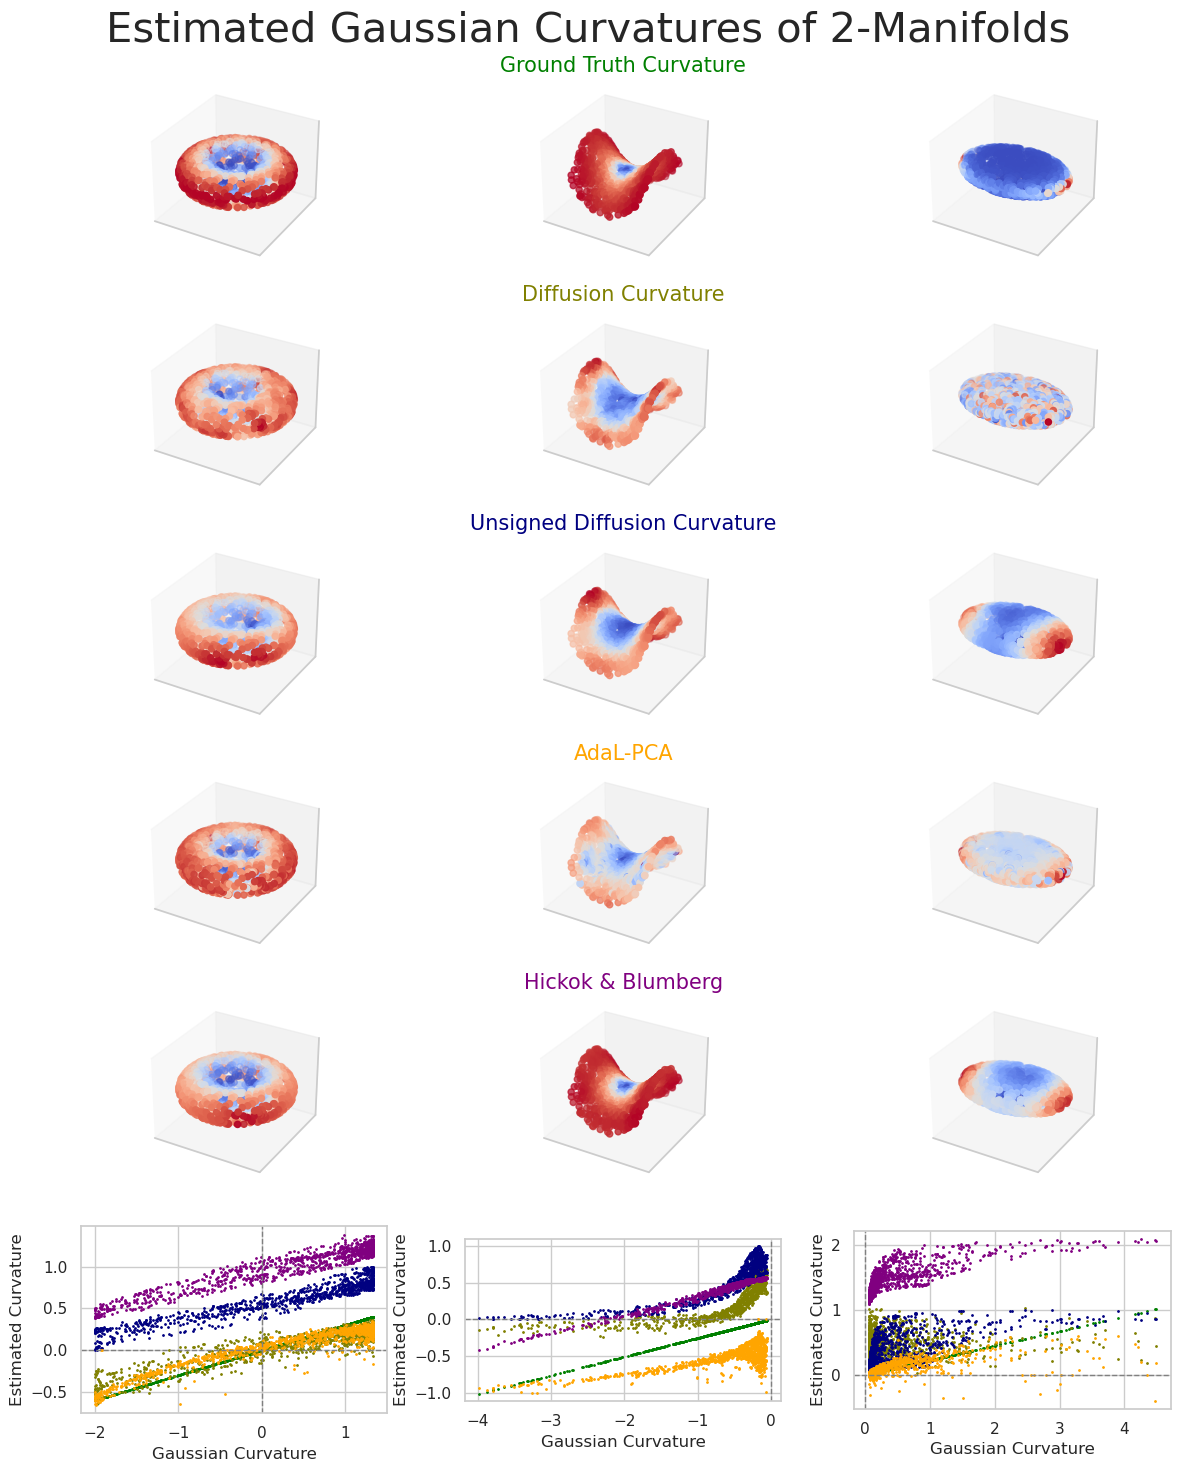
\includegraphics{index_files/figure-latex/..-nbs-experiments-2a2-toy-manifolds-comparison-fig-2-manifolds-visual-comparison-output-1.png}

}

\caption{\label{fig-2-manifolds-visual-comparison}Diffusion Curvature vs
Gaussian Curvature on 2-Manifolds.}

\end{figure}%

\textsubscript{Source:
\href{https://professorwug.github.io/diffusion-curvature//home/piriac/Pumberton/Workshop/21-SUMRY-Curvature/diffusion-curvature/nbs/experiments/2a2-toy-manifolds-comparison.ipynb.html\#cell-fig-2-manifolds-visual-comparison}{Standard
libraries}}

The second subtly emerges in the context of related methods. Everything
pictured does an excellent job of coloring the toy manifolds. But
looking beyond this, \emph{what matters?} Most methods don't care about
the precise magnitude -- or even exactly matching the correlations, as
in the ellipsoid\ldots{} \%\% mean vs gaussian curvature, and uniqueness
of definitions\%\%

All of these methods in Figure~\ref{fig-2-manifolds-visual-comparison}
perform well on well-sampled noiseless toy manifolds. In Table
\textbf{?@fig-2-manifolds-noise-table}, we see the results of adding
Gaussian noise to each manifold.

\subsubsection{Differentiating Sign in High
Dimensions}\label{differentiating-sign-in-high-dimensions}

Most existing methods only quantify their performance in high dimensions
on one or two test cases.

\begin{figure}[H]

\centering{

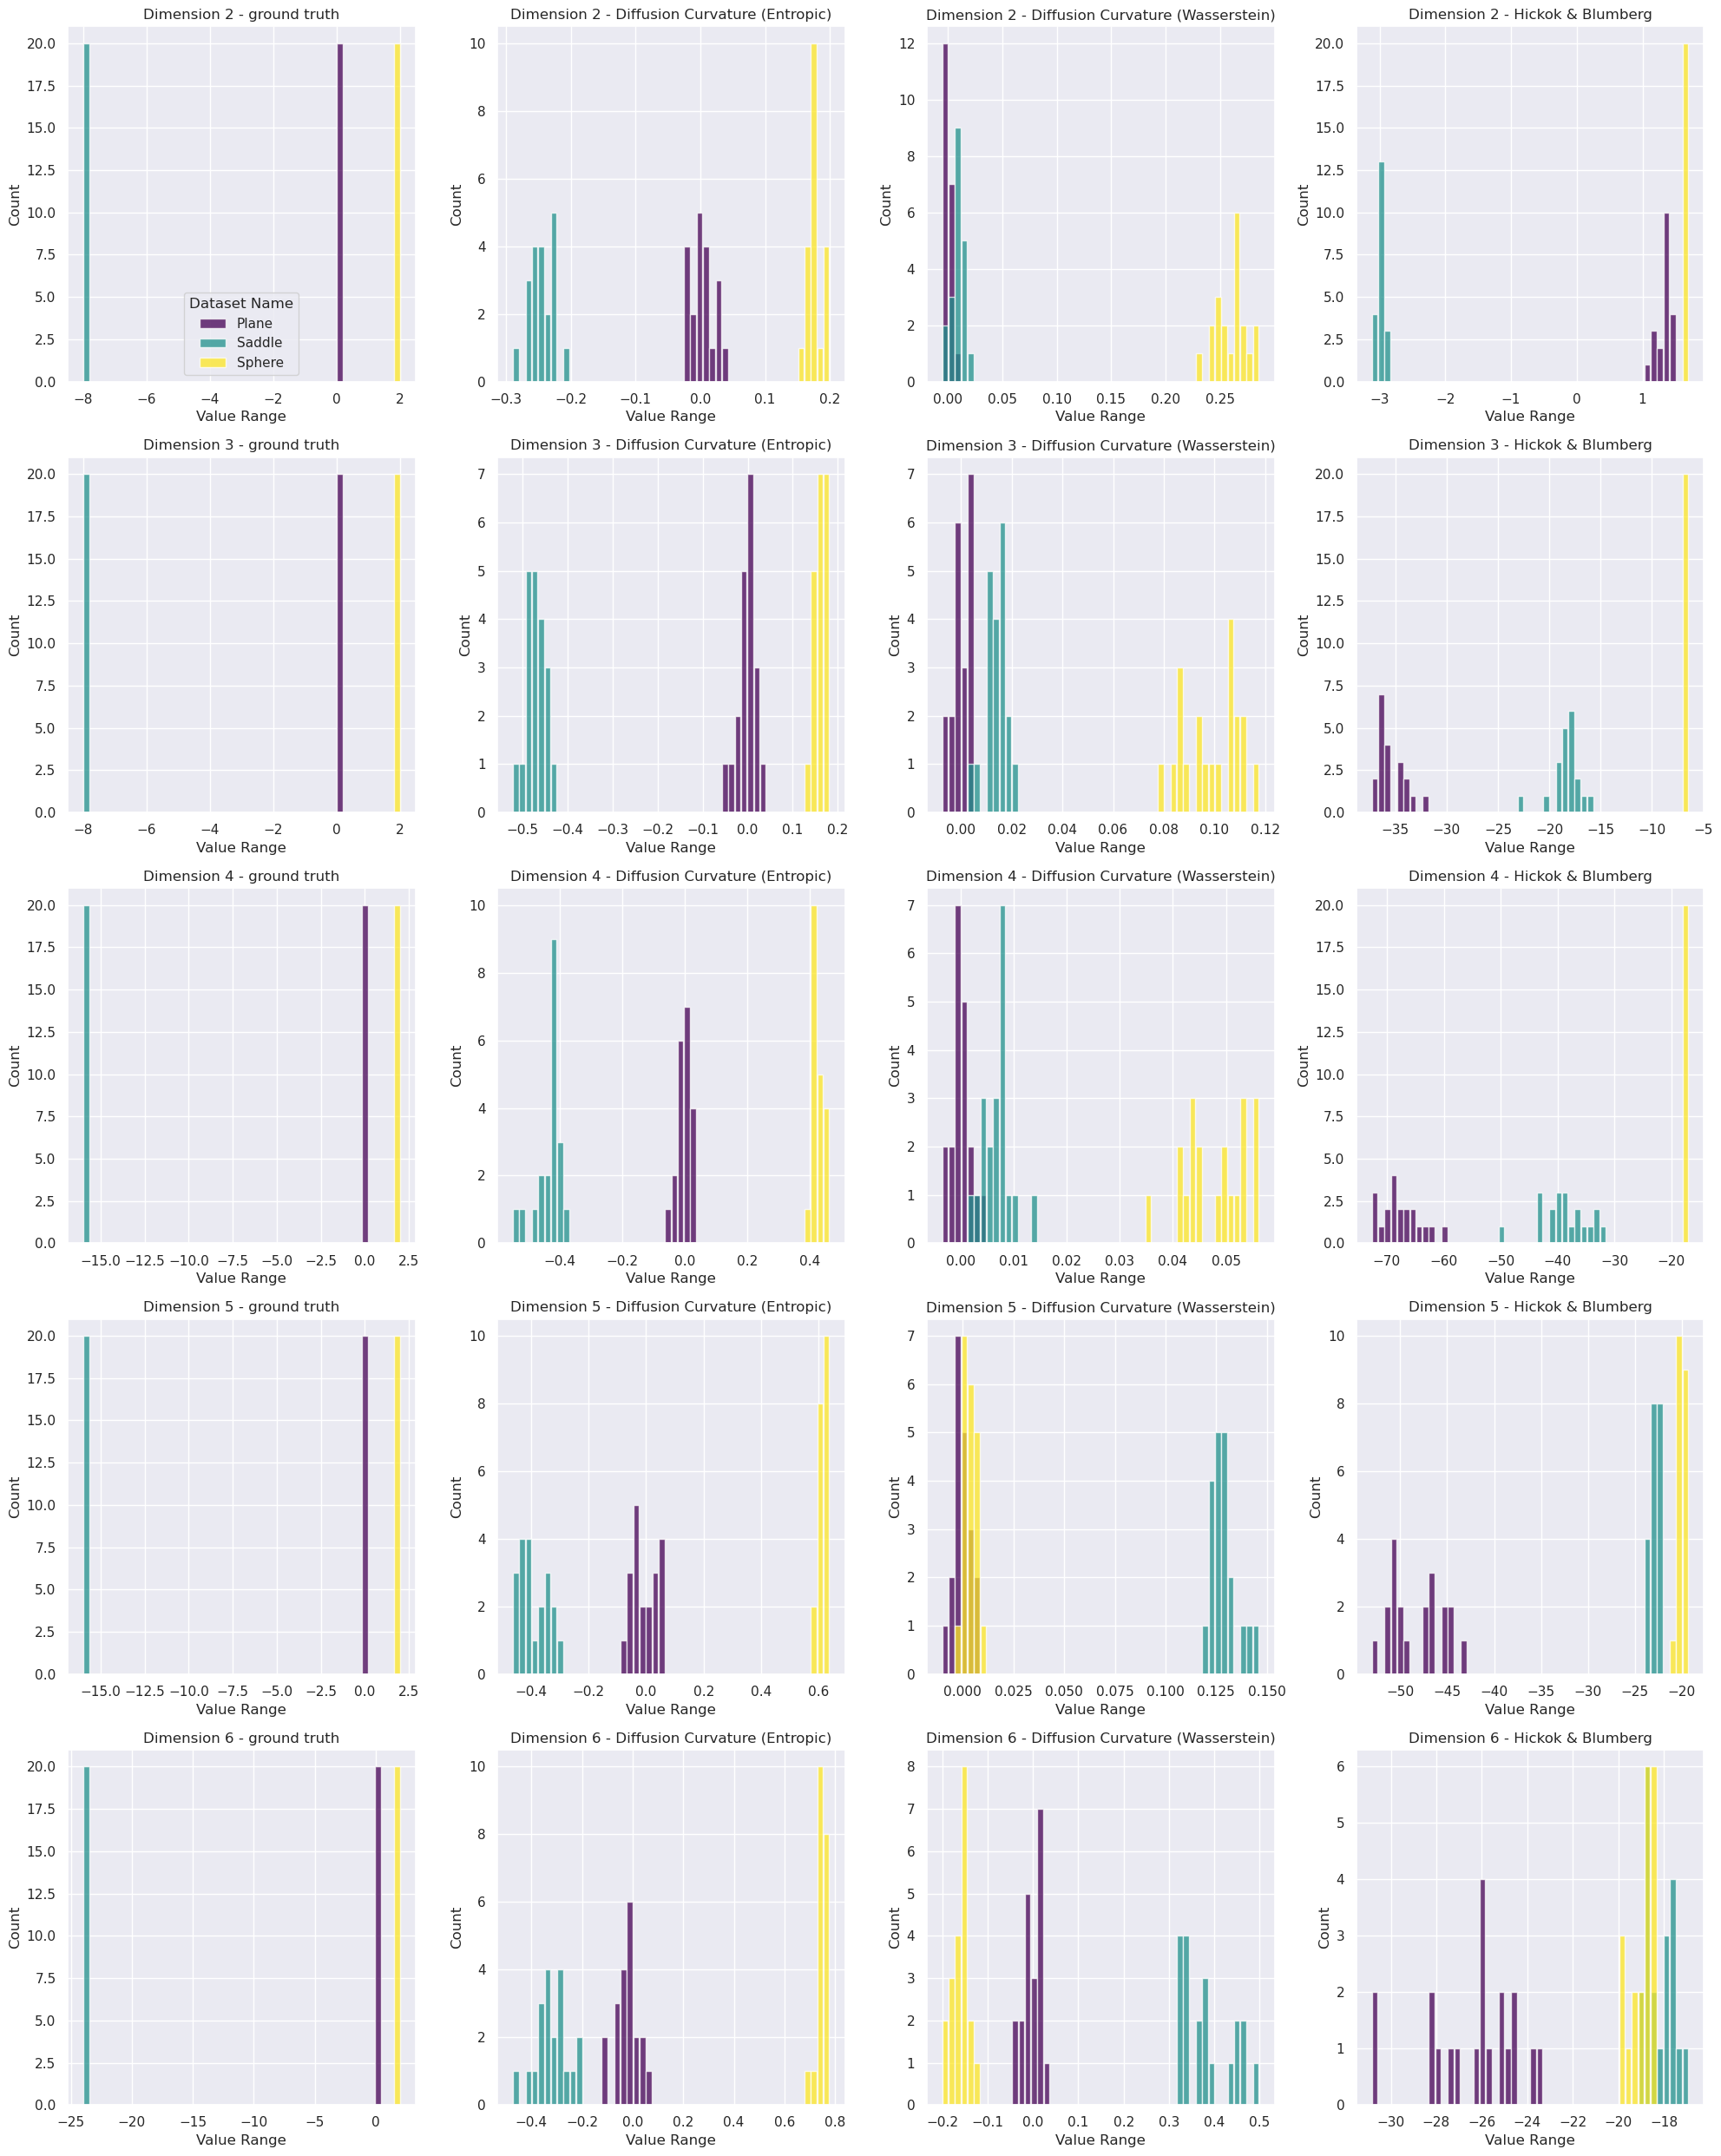
\includegraphics{index_files/figure-latex/..-nbs-experiments-2f-sign-prediction-tests-fig-sadspheres-output-1.png}

}

\caption{\label{fig-sadspheres}Predicted curvatures of Saddles and
Spheres in dimensions 2-6. Diffusion Curvature robustly distinguishes
between the signs of the data, even in high dimensions, and with
relative sparsity.}

\end{figure}%

\textsubscript{Source:
\href{https://professorwug.github.io/diffusion-curvature//home/piriac/Pumberton/Workshop/21-SUMRY-Curvature/diffusion-curvature/nbs/experiments/2f-sign-prediction-tests.ipynb.html\#cell-fig-sadspheres}{Standard
libraries}}

\subsection{Loss Landscapes}\label{loss-landscapes}

\subsection{Curvature as a TDA
Filtration}\label{curvature-as-a-tda-filtration}

\section{Related Work}\label{related-work}

\subsection{Foreman Ricci Curvature}\label{foreman-ricci-curvature}

\subsection{Hickock \& Blumberg's Volume Comparison
Curvature}\label{hickock-blumbergs-volume-comparison-curvature}

\section{Conclusion}\label{conclusion}

\section*{References}\label{references}
\addcontentsline{toc}{section}{References}

\phantomsection\label{refs}
\begin{CSLReferences}{1}{0}
\bibitem[\citeproctext]{ref-bhaskar2022DiffusionCurvatureEstimating}
Bhaskar, Dhananjay, Kincaid MacDonald, Oluwadamilola Fasina, Dawson
Thomas, Bastian Rieck, Ian Adelstein, and Smita Krishnaswamy. 2022.
{``Diffusion Curvature for Estimating Local Curvature in High
Dimensional Data.''} \emph{Advances in Neural Information Processing
Systems} 35: 21738--49.
\url{https://proceedings.neurips.cc/paper_files/paper/2022/hash/88438dc62fc5c8777e2b5f1b4f6d37a2-Abstract-Conference.html}.

\bibitem[\citeproctext]{ref-2021BishopGromovInequality}
{``Bishop--{Gromov} Inequality.''} 2021. In \emph{Wikipedia}.
\url{https://en.wikipedia.org/w/index.php?title=Bishop\%E2\%80\%93Gromov_inequality&oldid=1059331416}.

\bibitem[\citeproctext]{ref-coifman2006DiffusionMaps}
Coifman, Ronald R., and Stéphane Lafon. 2006. {``Diffusion Maps.''}
\emph{Applied and Computational Harmonic Analysis}, Special {Issue}:
{Diffusion Maps} and {Wavelets}, 21 (1): 5--30.
\url{https://doi.org/10.1016/j.acha.2006.04.006}.

\bibitem[\citeproctext]{ref-hickok2023IntrinsicApproachScalarCurvature}
Hickok, Abigail, and Andrew J. Blumberg. 2023. {``An {Intrinsic
Approach} to {Scalar-Curvature Estimation} for {Point Clouds}.''} arXiv.
\url{https://doi.org/10.48550/arXiv.2308.02615}.

\bibitem[\citeproctext]{ref-huguet2023HeatDiffusionPerspective}
Huguet, Guillaume, Alexander Tong, Edward De Brouwer, Yanlei Zhang, Guy
Wolf, Ian Adelstein, and Smita Krishnaswamy. 2023. {``A {Heat Diffusion
Perspective} on {Geodesic Preserving Dimensionality Reduction}.''} May
30, 2023. \url{https://doi.org/10.48550/arXiv.2305.19043}.

\bibitem[\citeproctext]{ref-maaten2008VisualizingDataUsing}
Maaten, Laurens van der, and Geoffrey Hinton. 2008. {``Visualizing
{Data} Using t-{SNE}.''} \emph{Journal of Machine Learning Research} 9
(86): 2579--2605. \url{http://jmlr.org/papers/v9/vandermaaten08a.html}.

\bibitem[\citeproctext]{ref-moon2019VisualizingStructureTransitions}
Moon, Kevin R., David van Dijk, Zheng Wang, Scott Gigante, Daniel B.
Burkhardt, William S. Chen, Kristina Yim, et al. 2019. {``Visualizing
Structure and Transitions in High-Dimensional Biological Data.''}
\emph{Nature Biotechnology} 37 (12, 12): 1482--92.
\url{https://doi.org/10.1038/s41587-019-0336-3}.

\bibitem[\citeproctext]{ref-ollivier2009RicciCurvatureMarkov}
Ollivier, Yann. 2009. {``Ricci Curvature of {Markov} Chains on Metric
Spaces.''} \emph{Journal of Functional Analysis} 256 (3): 810--64.
\url{https://doi.org/10.1016/j.jfa.2008.11.001}.

\bibitem[\citeproctext]{ref-saloff-coste2010HeatKernelIts}
Saloff-Coste, Laurent. 2010. {``The Heat Kernel and Its Estimates.''} In
\emph{Advanced {Studies} in {Pure Mathematics}}, 405--36. Kyoto
University, Japan. \url{https://doi.org/10.2969/aspm/05710405}.

\bibitem[\citeproctext]{ref-steinerberger2022CurvatureGraphsEquilibrium}
Steinerberger, Stefan. 2022. {``Curvature on {Graphs} via {Equilibrium
Measures}.''} September 5, 2022.
\url{https://doi.org/10.48550/arXiv.2202.01658}.

\bibitem[\citeproctext]{ref-sturm2006GeometryMetricMeasure}
Sturm, Karl-Theodor. 2006. {``On the Geometry of Metric Measure
Spaces.''} \emph{Acta Mathematica} 196 (1): 65--131.
\url{https://doi.org/10.1007/s11511-006-0002-8}.

\bibitem[\citeproctext]{ref-tong2021DiffusionEarthMovera}
Tong, Alexander Y., Guillaume Huguet, Amine Natik, Kincaid Macdonald,
Manik Kuchroo, Ronald Coifman, Guy Wolf, and Smita Krishnaswamy. 2021.
{``Diffusion {Earth Mover}'s {Distance} and {Distribution
Embeddings}.''} In \emph{Proceedings of the 38th {International
Conference} on {Machine Learning}}, 10336--46. PMLR.
\url{https://proceedings.mlr.press/v139/tong21a.html}.

\bibitem[\citeproctext]{ref-tong2021DatadrivenLearningGeometric}
Tong, Alexander, Frederick Wenkel, Kincaid Macdonald, Smita
Krishnaswamy, and Guy Wolf. 2021. {``Data-Driven Learning of Geometric
Scattering Modules for Gnns.''} In \emph{2021 {IEEE} 31st {International
Workshop} on {Machine Learning} for {Signal Processing} ({MLSP})}, 1--6.
IEEE. \url{https://ieeexplore.ieee.org/abstract/document/9596169/}.

\end{CSLReferences}



\end{document}
